\documentclass[tikz,border=8pt]{standalone}
\usepackage{amsmath}
\usetikzlibrary{arrows.meta}

\begin{document}
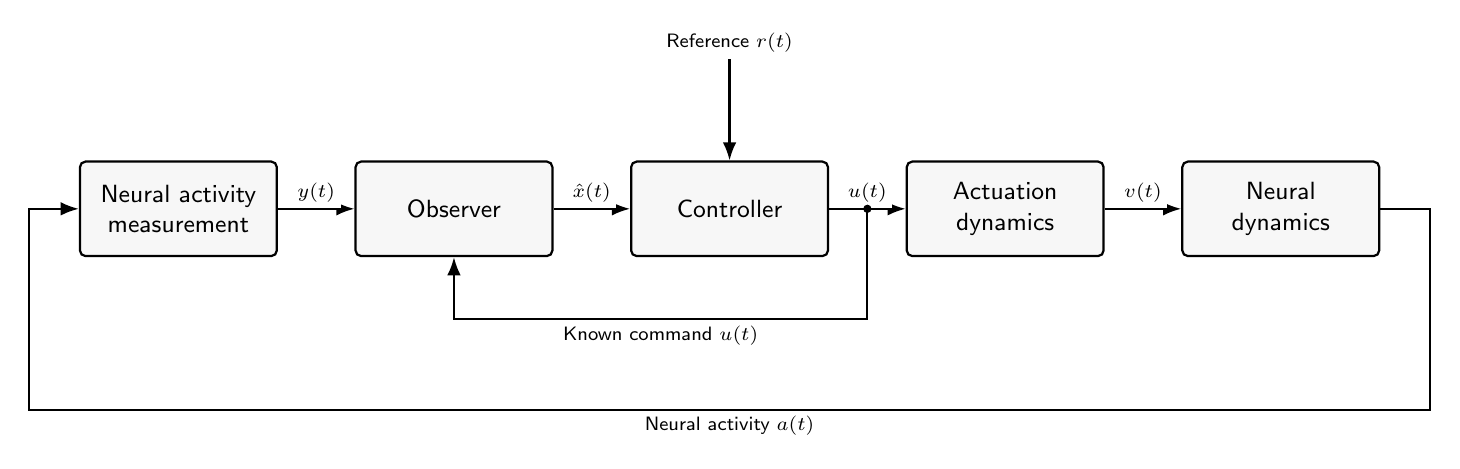
\begin{tikzpicture}[
  font=\sffamily\small,
  block/.style={draw,thick,rounded corners=2pt,minimum width=2.5cm,
    minimum height=1.2cm,align=center,fill=black!3},
  signal/.style={-{Latex[length=2.3mm]},thick},
  label/.style={font=\sffamily\scriptsize,align=center,fill=white,inner sep=2pt}
]
  \node[block] (measurement) at (0,0) {Neural activity\\measurement};
  \node[block] (observer) at (3.5,0) {Observer};
  \node[block] (controller) at (7,0) {Controller};
  \node[block] (actuation) at (10.5,0) {Actuation\\dynamics};
  \node[block] (neural) at (14,0) {Neural\\dynamics};

  \draw[signal] (measurement.east) -- node[above,label] {$y(t)$}
    (observer.west);
  \draw[signal] (observer.east) -- node[above,label] {$\hat{x}(t)$}
    (controller.west);
  \draw[signal] (controller.east) -- node[above,label] {$u(t)$}
    coordinate[midway] (command) (actuation.west);
  \draw[signal] (actuation.east) -- node[above,label] {$v(t)$}
    (neural.west);

  \draw[signal] (7,1.9) node[above,label] {Reference $r(t)$}
    -- (controller.north);

  \fill (command) circle (1.5pt);
  \draw[signal] (command) -- (8.75,-1.4)
    -- node[below,label] {Known command $u(t)$} (3.5,-1.4)
    -- (observer.south);

  \draw[signal] (neural.east) -- (15.9,0) -- (15.9,-2.55)
    -- node[below,label] {Neural activity $a(t)$} (-1.9,-2.55)
    -- (-1.9,0) -- (measurement.west);
\end{tikzpicture}
\end{document}
